\documentclass[article,A4,12pt]{llncs}

% Conditional compilation.
% NOTE: If you set fullversionfalse, just compile ONCE so that TOC stays unchanged.
\newif\iffullversion
\fullversiontrue
%\fullversionfalse

\usepackage[T1]{fontenc}
\usepackage{amsmath}
\usepackage{amssymb}
\usepackage{color}
\usepackage{amsfonts}
\usepackage{mathrsfs, bm}

\usepackage{graphicx}
\usepackage{tabularx}
\usepackage{subfig}
\usepackage{epsf,times}
\usepackage{color}
\usepackage{wrapfig}
\usepackage{cases}
\usepackage{multicol}

\usepackage[T1]{fontenc}
%\newcommand{\tmname}[1]{\textsc{#1}}
%\newcommand{\tmop}[1]{\ensuremath{\operatorname{#1}}}
%\newcommand{\tmsamp}[1]{\textsf{#1}}
%\newcommand{\tmtextsc}[1]{{\scshape{#1}}}
%\newcommand{\tmtextsl}[1]{{\slshape{#1}}}
%\newcommand{\tmtexttt}[1]{{\ttfamily{#1}}}

\leftmargin=0.0cm
\oddsidemargin=0.5cm
\evensidemargin=0.5cm
\topmargin=0cm
\textwidth=16.0cm
%\textheight=21.5cm
\textheight=20.0cm
\pagestyle{plain}
\setlength{\columnsep}{20pt}

\def\m{\mathbf{m}}
\def\H{\mathbf{H}}
\def\E{\mathbf{E}}
\newcommand{\vepsi}{{\varepsilon}}
\def\hnorm#1#2{\vert\,#1\,\vert_{#2}}
\newcommand{\R}{{\mathbb R}}
\newcommand{\Sph}{{\mathbb S}}
\def\x{\mathbf{x}}
\def\hvec{\overline{\mathbf{h}}}
\def\evec{\overline{\mathbf{e}}}

\newcommand{ \etal}{\mbox{\emph{et al. }}}

\newcommand\vect[1]{\mbf{#1}}
\newcommand{\mbf}[1]{\mbox{\boldmath$#1$}} 
\newcommand{\RC}[1]{#1 $\times$ #1 $\times$ #1}
\def\um{$\mu$m}
\def\C{$^{\circ}\mathrm{C}$}

\newcommand{\Rmnum}[1]{\expandafter\@slowromancap\romannumeral #1@}

% DEFINITION OF CUSTOM FONT SIZE
\newcommand{\customfontA}{\fontsize{50}{55}\selectfont}
\newcommand{\customfontB}{\fontsize{14.4}{20}\selectfont}
\newcommand{\customfontC}{\fontsize{30}{35}\selectfont}

\DeclareMathAlphabet{\mathpzc}{OT1}{pzc}{m}{it}

\def\clovek#1{\noindent\bgroup\vbox{\noindent#1}\egroup\vskip1em}

% TO INPUT BACKGROUND IMAGE
%\usepackage{eso-pic}
%\newcommand\BackgroundPic{
%\put(0,0){
%\parbox[b][\paperheight]{\paperwidth}{
%\vfill
%\centering
%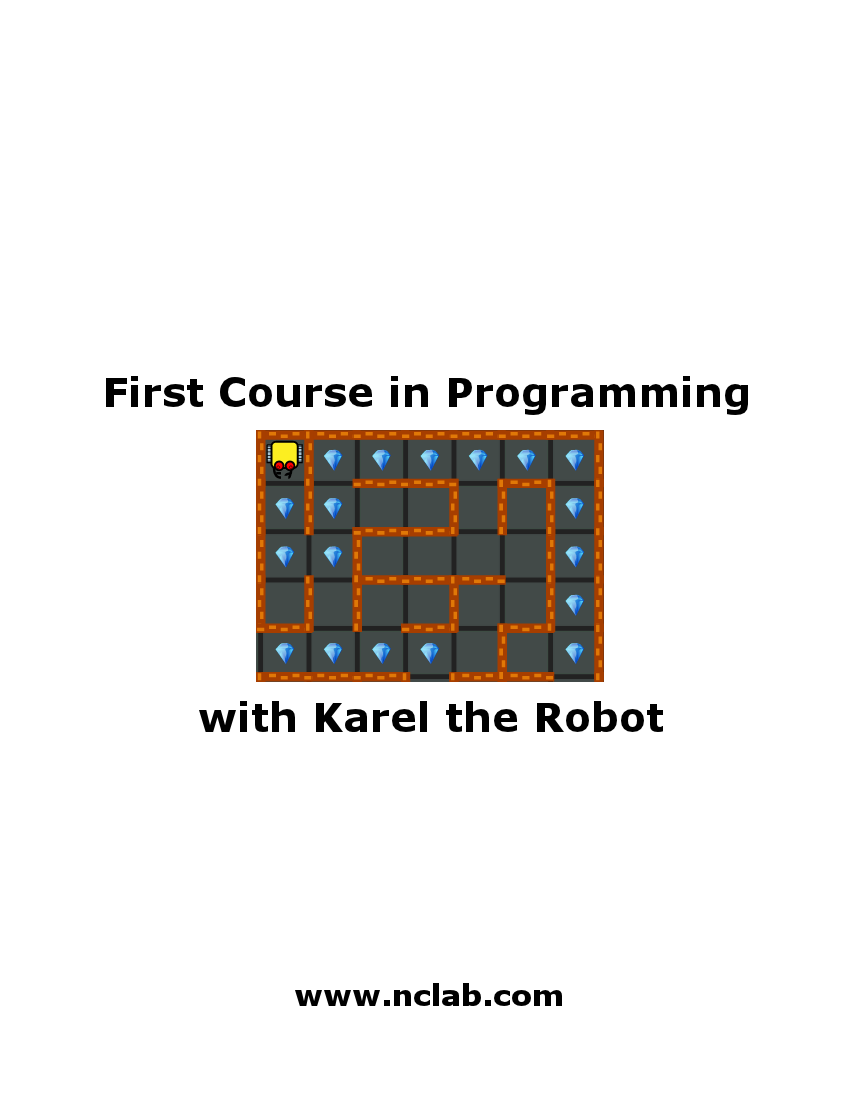
\includegraphics[width=\paperwidth,height=\paperheight]{img/karel-frontpage.png}
%%\includegraphics[width=\paperwidth,height=\paperheight]{img/background.jpg}
%\vfill
%}}}

\begin{document}

% INPUTTING BACKGROUND IMAGE
%\AddToShipoutPicture{\BackgroundPic}
%\vbox{}
%\pagestyle{empty}
%\newpage
%\textwidth=15.5cm
%\ClearShipoutPicture
%\newpage

%%%%%%%%%%%%%%%%%%%%%%%%%%%%%%%%%%%%%%%%%%%%%%%%%%%%%%%%%%%%%%%%%%%%%%%%%
\pagestyle{empty}

\vbox{}
\begin{figure}[!ht]
%\hspace{-4mm}

\includegraphics[width=8cm]{imgp/logo.png}
\vspace{18mm}
\end{figure}
\vbox{}
\vspace{0.5cm}

\begin{center}
{\huge \bf First Course in Programming}
\end{center}

\begin{figure}[!ht]
\begin{center}
\vspace{-6mm}
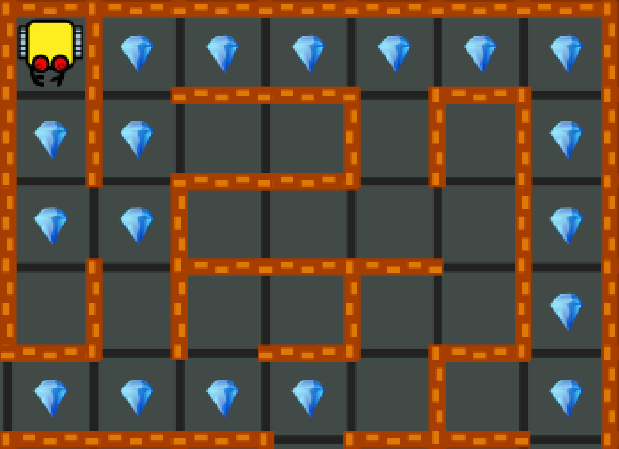
\includegraphics[width=0.26\textheight]{imgk/karel-logo.png}\ \ \ \ \ \ 
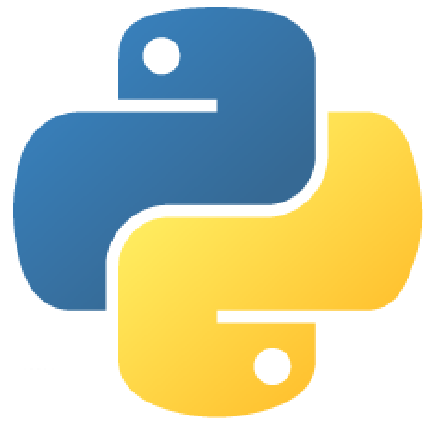
\includegraphics[width=0.2\textheight]{imgp/python-logo.png}
\vbox{}
\vspace{-9mm}
\end{center}
\end{figure}
\begin{center}
{\huge \bf with Karel the Robot and Python}
\end{center}
\vbox{}
\vspace{1cm}
\begin{center}
\iffullversion
\else
\centerline{\huge \color{red}{PREVIEW}}
\fi
\vfill
{\large
{\bf Pavel Solin}, University of Nevada, Reno\\
{\bf Salih Dede}, Coral Academy of Science, Reno
}
\end{center}
\newpage
\vbox{}
\vfill
\begin{center}
{
The textbook {\em Intro to Programming with Karel the Robot and Python} 
can be ordered at {\tt http://introtoprogramming.net}. The textbook 
is also available as part of the NCLab course {\em Intro to Programming} 
that can be purchased at {\tt http://introtoprogramming.net}.
Unauthorized copying and sharing is prohibited.
}
\vfill

Copyright 2012 FEMhub Inc. All rights reserved.
\end{center}


\newpage
%{\ }
\setcounter{tocdepth}{2}
\tableofcontents
%\pagestyle{plain}

\newpage

\pagestyle{plain}
\setcounter{page}{1}

%%%%%%%%%%%%%%%%%%%%%%%%%%%%%%%%%%%%%%%%%%%%%%%%%%%%%%%%%%%%%%%%%%%%%%%%%
\pagestyle{plain}
\setcounter{page}{1}
\section*{Foreword}
This course provides a gentle yet efficient and comprehensive introduction to modern algorithmic 
design and computer programming. It covers two programming languages -- {\em Karel the Robot} 
and {\em Python}. Karel the Robot is a famous 
educational programming language that was created at the Stanford University. It has a playful 
appearance, and using a handful of simple commands it helps students to develop advanced algorithmic 
skills quickly. Python is a modern high-level dynamical programming language that is widely 
used in business, science, and engineering applications. It is much easier to learn than C, C++ or 
Java.

Starting with Karel the Robot, students discover principles of computer programming effortlessly,
without being exposed to technical details of conventional programming languages.
Could such an introduction be done with a conventional programming language? Yes, but 
it would be obscurred and slowed down by technicalities, not mentioning that it would 
not be fun. The course starts out in Manual mode (Level 0) where the robot can be guided via 
clicking on five buttons {\em Go} (make one step forward), {\em Left} (turn left), {\em Right} 
(turn right), {\em Put} (put a gem on the groud) and {\em Get} (pick up a gem from the ground). 

\begin{figure}[!ht]
\begin{center}
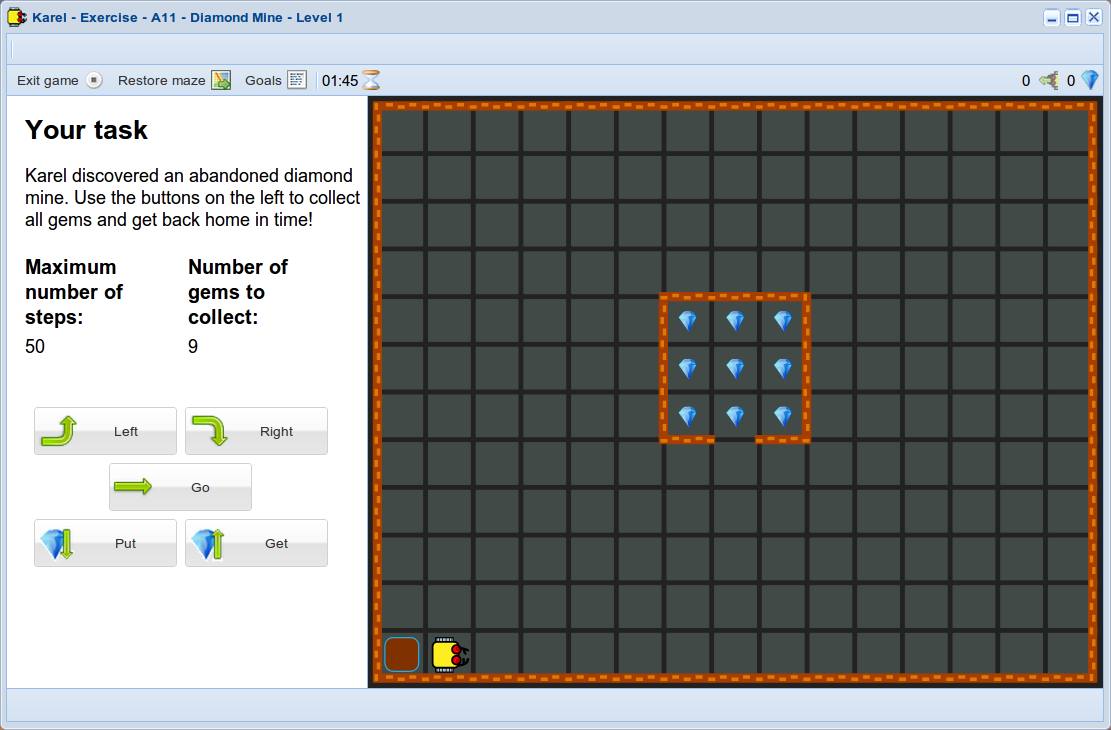
\includegraphics[width=0.8\textwidth]{imgk/fore-1.png}
\end{center}
\vspace{-2mm}
\caption{Sample game {\em Diamond Mine} in Manual mode.}
\label{fig:f1}
\vspace{-4mm}
\end{figure}
\noindent
In the next stage which is called {\em Bridge to Programming} students keep solving 
similar problems, but they type the commands 
{\tt go}, {\tt left}, {\tt right}, {\tt put} and {\tt get} instead of clicking on the 
corresponding buttons. This breaks the ice!

The need for higher functionality such as loops, conditions, and custom commands arises 
naturally as game goals get more challenging. 
Students understand quickly that it helps them to break complex tasks into smaller 
ones. {\em This is the most important principle of computer 
programming.} The textbook is written by programming experts, so in addition to the 
standard skills the students also learn a lot about good and bad programming practices.

\begin{figure}[!ht]
\begin{center}
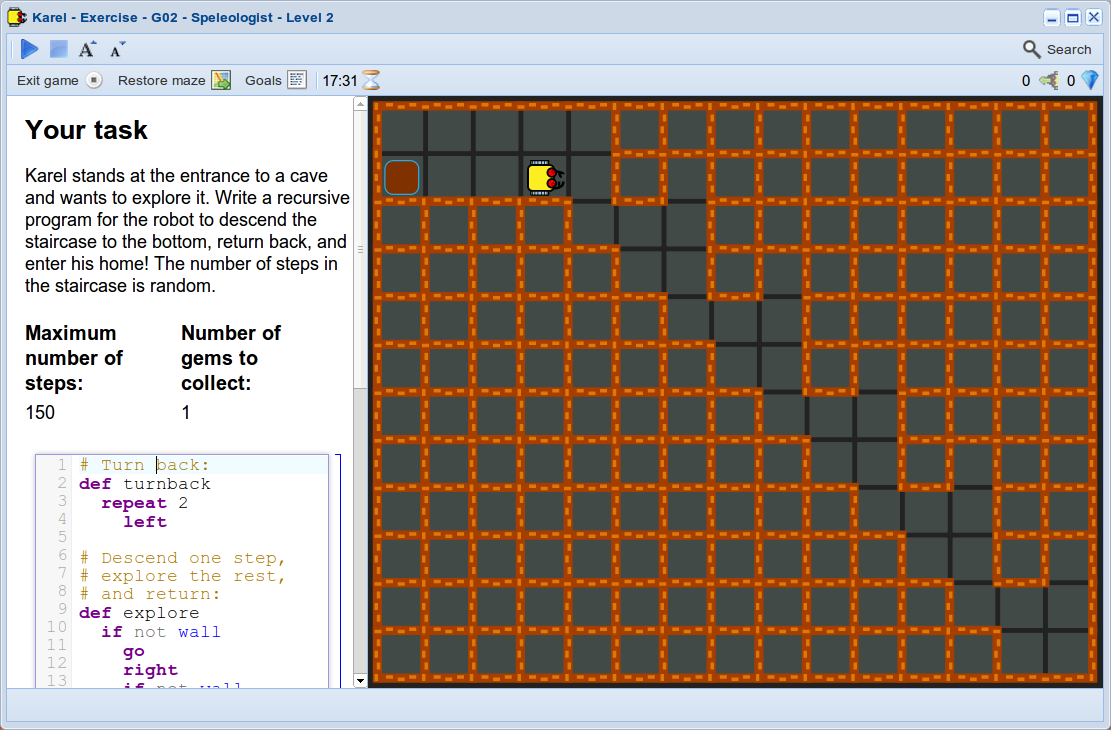
\includegraphics[width=0.8\textwidth]{imgk/fore-2.png}
\end{center}
\vspace{-2mm}
\caption{Sample game {\em Speleologist} in Programming mode.}
\label{fig:f2}
\vspace{-4mm}
\end{figure}
\noindent
The syntax of Karel the Robot is very close to Python -- in fact Python feels like Karel's
older brother. The transition from Karel to Python is as seamless as the transition from 
one Karel's Level to another. 
In Python, students continue building their skills in the same way they did with Karel. 
They learn more advanced concepts including mathematical operations, plotting, local and 
global variables, strings, tuples, lists, dictionaries, and others. They get to solve 
realistic problems, but Python is still a lot of fun. 

A very strong aspect of Python programming are its libraries. There is a Standard Library which 
contains many build-in functions that are not present in lower-level languages such as 
Java, C, C++ or Fortran. Python also has very powerful scientific libraries including 
Scipy, Numpy, Matplotlib, Pylab, Sympy and others. With these, students can start solving 
real scientific and engineering problems. These libraries are introduced at the end of this 
course.  




%Taking this course will make it much easier 
%for you to learn Python, C, C++ and other advanced programming languages. In particular we 
%recommend that after Karel you continue with Python, a powerful programming 
%language that is used across all science and engineering areas, and yet it is 
%technically simpler to handle than C or C++. 



\part{Karel the Robot}

\input karel.tex

\part{Introduction to Python}

\input python.tex

\section{What next?}

Congratulations, you made it! We hope that you enjoyed the textbook and the 
exercises. If you can think of any way to improve the application Karel the 
Robot or this tutorial, we would be very happy to hear from you. If you 
have an interesting new game or exercises for Karel, please let us know as well. 

Although you may feel like an Almighty Programmer right now, we would
recommend staying humble. Even the most experienced programmers are
learning new things all the time. There is much more to Python that 
we managed to cover in this introductory textbook. You already know 
about the Internet resources where you can learn more.  

Alternatively, you may dive into a next programming language! We would 
recommend Javascript since this is the most popular language for web 
development. Of course there are many more languages to explore, including 
C/C++, Java, Perl, Ruby, Lua and others.\\

\noindent
In any case, our team wishes you good luck, and keep us in your 
favorite bookmarks! \\

\hbox{} \hfill{} Your NCLab Team




\end{document}
